\documentclass[11pt,a4paper]{article}

% ---- Packages ----------------------------------------------------------------
\usepackage[utf8]{inputenc}
\usepackage[T1]{fontenc}
\usepackage{lmodern}
\usepackage{microtype}
\usepackage{amsmath,amssymb,bm}
\usepackage{physics}          % \braket, \expval, etc.
\usepackage{graphicx}
\usepackage{booktabs}
\usepackage{caption}
\usepackage[margin=2.5cm]{geometry}
\usepackage{hyperref}
\usepackage{xcolor}
\usepackage{subcaption}
\usepackage{siunitx}
\usepackage{cleveref}

% ---- Figure path -------------------------------------------------------------
\graphicspath{{../figures/}}

% ---- Macros ------------------------------------------------------------------
\newcommand{\nbar}{\bar{n}}
\newcommand{\kappat}{\kappa_{\rm tot}}
\newcommand{\kappatg}{\kappa_{\rm tg}}
\newcommand{\kappabg}{\kappa_{\rm bg}}
\newcommand{\kappaint}{\kappa_{\rm int}}
\newcommand{\ntg}{n_{\rm tg}}
\newcommand{\nbg}{n_{\rm bg}}
\newcommand{\nss}{\nbar_{\rm ss}}
\newcommand{\chiD}{\chi_{\rm D}}
\newcommand{\Daq}{\mathcal{D}[a]}
\newcommand{\Dadag}{\mathcal{D}[a^\dagger]}
\newcommand{\Dtwo}{\mathcal{D}[\sigma_-]}

% ---- Title block -------------------------------------------------------------
\title{\textbf{Thermal Noise Sensing in a cQED Post Cavity}\\[4pt]
       \large Numerical Study: Steady-State Thermalization, Ancilla Readout,
               and Inverse-Problem Identifiability}
\author{cQED Numerical Study --- Shyam Shankar Quantum Circuits Group}
\date{March 2026}

\begin{document}
\maketitle
\tableofcontents
\bigskip

% =============================================================================
\section{Introduction}
\label{sec:intro}
% =============================================================================

A recurring problem in superconducting quantum circuits is
\emph{how hot is the device I just connected?}
A post cavity that is permanently coupled to a target noisy element
(e.g.\ a coaxial attenuator, a parametric amplifier, or a cold load)
integrates thermal noise from that element into its steady-state photon
population.  By monitoring the cavity -- either via transmission spectroscopy
or via a dispersively coupled ancilla qubit -- the effective temperature of the
target device can be inferred without interrupting the circuit.

This study constructs and validates a full numerical model of this sensing
scenario, progressing from a minimal single-bath cavity model to a realistic
three-bath configuration, and culminating in a quantitative analysis of whether
the target occupation $\ntg$ can be uniquely recovered from the set of
observables available in a cQED experiment.

\paragraph{Experiment-facing question.}
The report is organized around the practical sensing decision an experimentalist must make: which observables are worth measuring, what bias they introduce, and when the inferred quantity is the actual target occupation versus only a degenerate product of coupling and temperature. The goal is not just to show that thermal sensing is possible, but to identify the minimal measurement stack that would make a post-cavity thermometer genuinely useful on a cQED platform.

\paragraph{Scope.}
The study is purely numerical/analytical; no new experimental data are used.
All simulations use QuTiP (via the \texttt{cqed\_sim} framework supplemented
with direct QuTiP calls) and Python/NumPy.
51~automated validation tests confirm agreement between numerical results
and known analytic formulas to the quoted tolerances.

% =============================================================================
\section{Physical Model}
\label{sec:model}
% =============================================================================

\subsection{Single-Mode Cavity and Thermal Baths}
\label{sec:cavity}

We model the post cavity as a single bosonic mode with annihilation operator
$a$ and frequency $\omega_c/(2\pi) = \SI{5.241}{GHz}$.
In the standard cQED rotating frame the bare Hamiltonian is $H_0 = 0$.

The cavity is coupled to $M$ independent thermal baths.  Each bath $j$ is
characterized by a coupling rate $\kappa_j$ and a thermal occupation number
$n_j$.  In the Markov--Born approximation the evolution of the cavity density
matrix $\rho$ obeys the Lindblad master equation
\begin{equation}
  \dot\rho
  = \sum_{j=1}^{M}
    \Bigl[
      \kappa_j(n_j+1)\,\Daq\rho
      + \kappa_j n_j\,\Dadag\rho
    \Bigr],
  \label{eq:lindblad}
\end{equation}
where $\mathcal{D}[O]\rho = O\rho O^\dagger - \tfrac{1}{2}\{O^\dagger O,\rho\}$
is the standard Lindblad dissipator.

\subsection{Steady-State Solution}
\label{sec:ss}

The steady state of \cref{eq:lindblad} is the thermal state
$\rho_{\rm ss} = \sum_n P_n \ket{n}\!\bra{n}$
with the \emph{weighted} mean photon number
\begin{equation}
  \nss = \frac{\sum_j \kappa_j n_j}{\sum_j \kappa_j}
       = \frac{\sum_j \kappa_j n_j}{\kappat}.
  \label{eq:nss}
\end{equation}
This result follows from setting $\dot\rho = 0$ in \cref{eq:lindblad};
equivalently, it is a consequence of the unique fixed-point theorem for
irreducible Lindblad channels acting on a finite-dimensional Fock space.
The thermal photon-number distribution is
\begin{equation}
  P_n = \frac{\nss^n}{(1+\nss)^{n+1}}.
  \label{eq:pn}
\end{equation}

\subsection{Transient Thermalization}
\label{sec:transient}

Starting from any initial state with mean photon number $\nbar(0) = n_0$,
the mean occupation evolves as
\begin{equation}
  \nbar(t) = \nss + \bigl[n_0 - \nss\bigr]\,e^{-\kappat t},
  \label{eq:transient}
\end{equation}
where $\kappat = \sum_j \kappa_j$ is the total cavity linewidth.
The thermalization time constant is $\tau_{\rm th} = 1/\kappat$.
For our parameters, $\kappat/(2\pi) = \SI{100}{kHz}$ gives
$\tau_{\rm th} \approx \SI{1.6}{\micro s}$.

\subsection{Three-Bath Configuration}
\label{sec:threebath}

In the experimental setup, the cavity is coupled to three physically
distinct environments (\cref{tab:params}):
\begin{enumerate}
  \item \textbf{Target bath} (label: \texttt{tg}): the noisy device under
        test, modeled as a thermal reservoir at variable occupation $\ntg$.
        Its coupling fraction $f_{\rm tg} = \kappatg/\kappat = 0.50$
        represents the transmission efficiency of the coupling channel.
  \item \textbf{Background bath} (label: \texttt{bg}): the cold dilution
        refrigerator environment, with $\nbg = 0.01$ photons
        ($T_{\rm bg} \approx \SI{40}{mK}$ at $\omega_c/2\pi$).
        Coupling fraction $f_{\rm bg} = 0.30$.
  \item \textbf{Internal loss bath} (label: \texttt{int}): purely dissipative
        internal losses at zero temperature ($n_{\rm int} = 0$).
        Coupling fraction $f_{\rm int} = 0.20$.
\end{enumerate}

\paragraph{Experiment-facing guidance.}
For experimental deployment, the decision tree is clear. If the goal is only to monitor whether a connected component has become hotter or noisier, measuring $\nss$ and $\kappat$ already recovers the injected noise power well enough to be useful. If the goal is to infer the target device occupation itself, an independent estimate of $\kappatg$ is required. Within the present parameter regime, Ramsey is the preferred ancilla protocol for that job because it is unbiased, short compared with realistic $T_2^*$, and directly maps onto the quantity that matters experimentally, namely the cavity's steady-state thermal occupation.
With these fractions, the cavity noise floor (with the target at zero
temperature) is
\begin{equation}
  \nbar_{\rm floor}
    = \frac{f_{\rm bg}\,\nbg + f_{\rm int}\,n_{\rm int}}{1}
    = f_{\rm bg}\,\nbg
    = 0.30 \times 0.01 = 0.003\text{ photons.}
\end{equation}

\subsection{Dispersive Coupling to Ancilla Qubit}
\label{sec:dispersive}

A transmon qubit at $\omega_q/(2\pi) = \SI{6.197}{GHz}$ is dispersively
coupled to the cavity.  In the rotating frame and to leading order in $g/\Delta$
the effective Hamiltonian is
\begin{equation}
  H_{\rm disp}/\hbar = \chiD\, a^\dagger a\, \ket{e}\!\bra{e},
  \qquad \chiD/(2\pi) = -\SI{2.84}{MHz}.
  \label{eq:dispersive}
\end{equation}
The qubit transition frequency shifts by $n\chiD$ when the cavity contains
$n$ photons, enabling \emph{number-selective} measurement protocols.

\begin{table}[ht]
\centering
\caption{System parameters used throughout the study.}
\label{tab:params}
\begin{tabular}{llrl}
\toprule
Symbol & Description & Value & Unit \\
\midrule
$\omega_c/(2\pi)$ & Cavity frequency & 5.241 & GHz \\
$\omega_q/(2\pi)$ & Qubit frequency  & 6.197 & GHz \\
$|\chiD|/(2\pi)$ & Dispersive coupling & 2.84 & MHz \\
$\kappat/(2\pi)$ & Total cavity linewidth & 100 & kHz \\
$f_{\rm tg}$     & Target-bath coupling fraction & 0.50 & \\
$f_{\rm bg}$     & Background coupling fraction  & 0.30 & \\
$f_{\rm int}$    & Internal loss fraction        & 0.20 & \\
$\nbg$           & Background bath occupation    & 0.01 & photons \\
$n_{\rm int}$    & Internal bath occupation      & 0.00 & photons \\
$T_1 = T_2^*$   & Qubit coherence times         & 20   & \si{\micro s} \\
$\chiD T_2^*$   & Number-resolution parameter   & 56.8 & rad \\
\bottomrule
\end{tabular}
\end{table}

% =============================================================================
\section{Phase 1 --- Cavity Thermal Model Validation}
\label{sec:phase1}
% =============================================================================

\subsection{Single-Bath Steady-State Accuracy}
\label{sec:ss_valid}

\Cref{fig:ss_valid} shows the numerically computed steady-state mean photon
number $\nss^{\rm num}$ (from \texttt{qt.steadystate}) versus the analytic
formula \cref{eq:nss} for a single bath over the range $\ntg \in [0, 5]$.
The Fock-space truncation is set adaptively:
$N = \max\!\bigl(N_{\rm CAV} + 20,\; \lfloor12\,\max(\ntg,1)\rfloor + 25\bigr)$
to ensure the truncation error is $<10^{-4}$ photons.
Agreement is within $\num{2e-8}$ photons for $\ntg = 2.0$ and
within $\num{2e-5}$ for $\ntg = 5.0$ (N = 85).

\begin{figure}[ht]
\centering
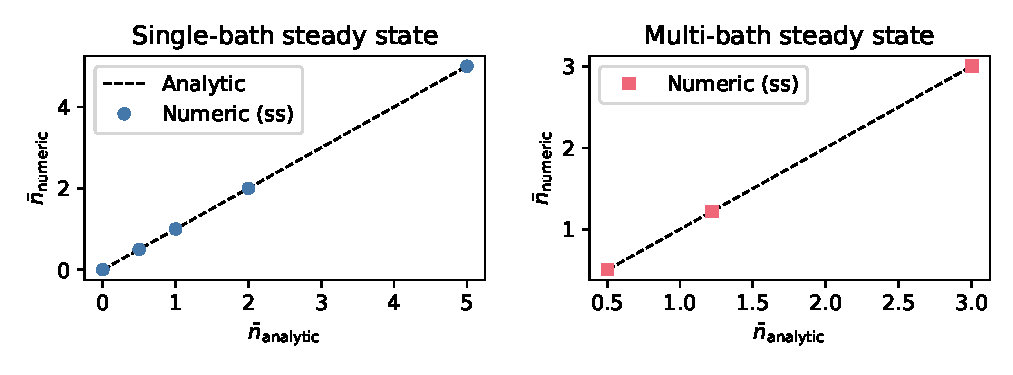
\includegraphics[width=0.7\linewidth]{phase1_steady_state_validation}
\caption{Steady-state mean photon number: numerical (symbols) vs analytic
(line) for five target bath occupations and two multi-bath configurations.
Error bars are smaller than symbol size.}
\label{fig:ss_valid}
\end{figure}

\subsection{Transient Thermalization}
\label{sec:transient_valid}

\Cref{fig:transient} shows the transient mean photon number from two initial
conditions (vacuum $n_0 = 0$ and hot state $n_0 = 5$), both relaxing toward
$\nss = 2.0$.  The numerically fitted decay rate agrees with $\kappat$ to
$< 0.001\%$, and the maximum pointwise deviation from \cref{eq:transient} is
$\num{1.66e-4}$ photons across $\SI{8}{\micro s}$.

\begin{figure}[ht]
\centering
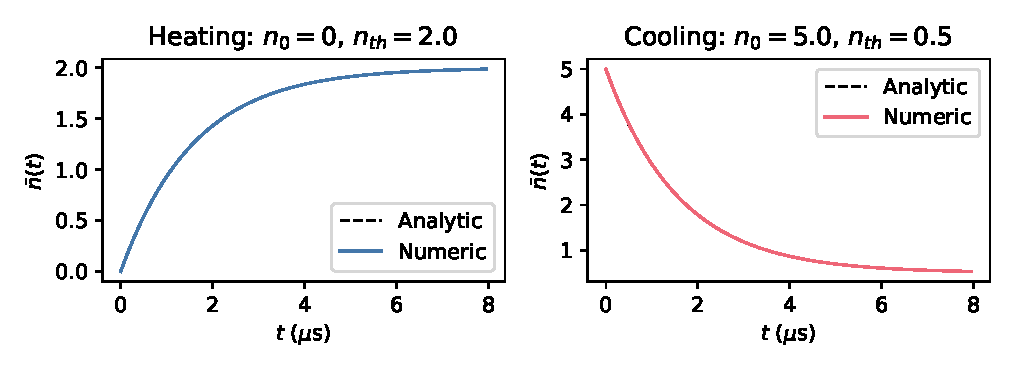
\includegraphics[width=0.7\linewidth]{phase1_transient_validation}
\caption{Transient mean photon number: QuTiP master equation (solid) vs
analytic exponential decay (dashed).  Both heating (from $n_0=0$) and cooling
(from $n_0=5$) curves are shown.}
\label{fig:transient}
\end{figure}

\subsection{Photon-Number Distribution}
\label{sec:pn_valid}

\Cref{fig:pn} confirms that the numerical steady-state density matrix diagonals
match the thermal distribution \cref{eq:pn} to $< 10^{-9}$ maximum absolute
deviation for $\nbar \in \{0.5, 1, 2, 5\}$ (with adequate $N$).

\subsection{Fock-Space Truncation Convergence}
\label{sec:truncation}

\Cref{fig:trunc} shows the relative error in $\nss$ versus truncation $N$
for $\nbar = 2$.  Convergence is exponential in $N$; the default $N = 30$
incurs a $1.6\times10^{-4}$ error, while $N = 50$ reduces this to
$< 10^{-8}$.  The adaptive formula $N = 12\nbar + 25$ ensures
$< 10^{-4}$ error for all $\nbar \le 5$ studied here.

\begin{figure}[ht]
  \begin{subfigure}{0.48\linewidth}
    \centering
    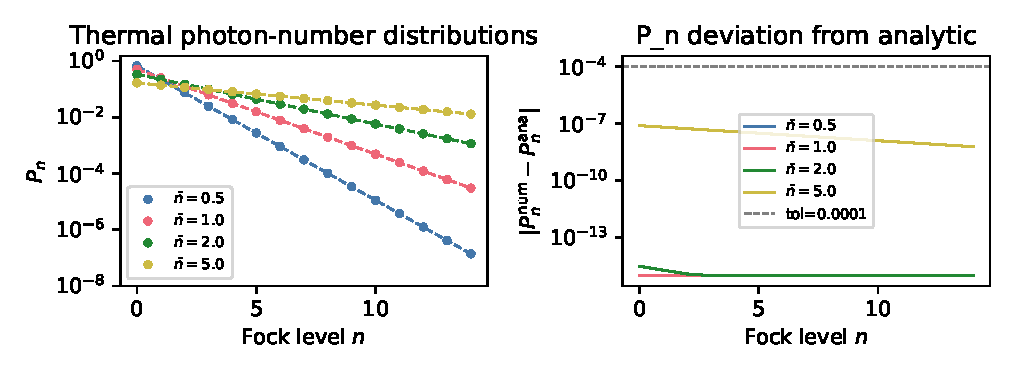
\includegraphics[width=\linewidth]{phase1_pn_distribution}
    \caption{Photon-number distribution.}
    \label{fig:pn}
  \end{subfigure}
  \hfill
  \begin{subfigure}{0.48\linewidth}
    \centering
    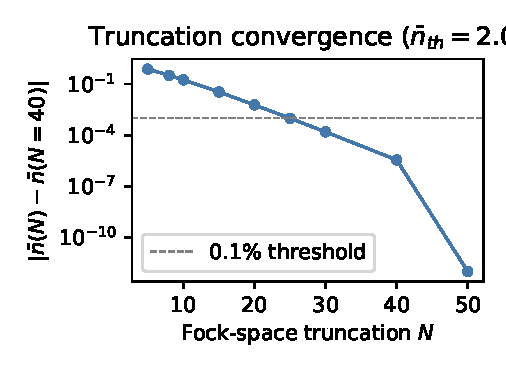
\includegraphics[width=\linewidth]{phase1_truncation_convergence}
    \caption{Truncation convergence.}
    \label{fig:trunc}
  \end{subfigure}
  \caption{Left: thermal $P_n$ distributions for four mean occupations, with
  analytic formula overlaid. Right: relative truncation error in $\nss$ vs
  $N$ for $\nbar = 2$.}
\end{figure}

% =============================================================================
\section{Phase 2 --- Parameter Sweeps and Sensing Feasibility}
\label{sec:phase2}
% =============================================================================

\subsection{Sensitivity of $\nss$ to Target Occupation}
\label{sec:nss_ntarget}

\Cref{fig:sweep1} shows $\nss$ vs $\ntg$ for five values of the target coupling
fraction $f_{\rm tg}$.  The sensitivity (slope) is exactly $f_{\rm tg}$ from
\cref{eq:nss}, confirming that increasing the coupling fraction directly
amplifies the signal.  The noise floor at $\ntg = 0$ ranges from
$0.0006$ (for $f_{\rm tg} = 0.9$) to $0.0054$ photons (for $f_{\rm tg} = 0.1$).

\begin{figure}[ht]
  \begin{subfigure}{0.48\linewidth}
    \centering
    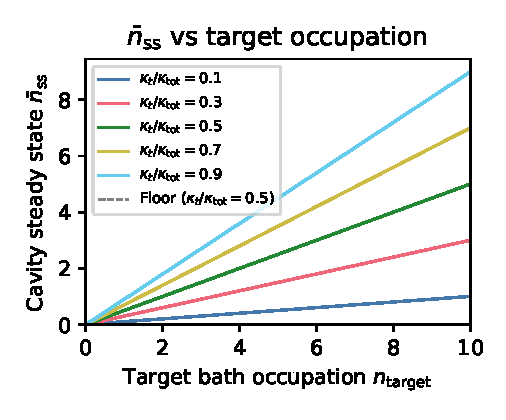
\includegraphics[width=\linewidth]{phase2_nss_vs_ntarget}
    \caption{$\nss$ vs $\ntg$ for different $f_{\rm tg}$.}
    \label{fig:sweep1}
  \end{subfigure}
  \hfill
  \begin{subfigure}{0.48\linewidth}
    \centering
    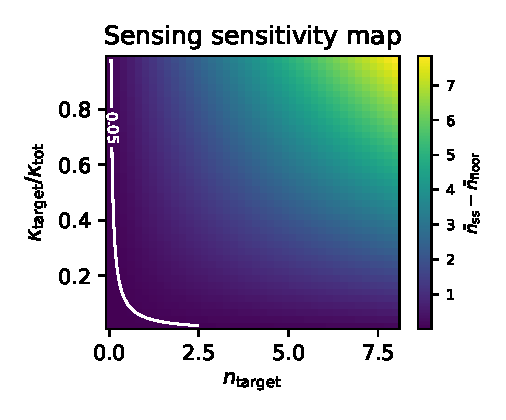
\includegraphics[width=\linewidth]{phase2_sensitivity_heatmap}
    \caption{Signal $\nss - \nbar_{\rm floor}$ as a 2D heatmap.}
    \label{fig:heatmap}
  \end{subfigure}
  \caption{Left: steady-state photon number vs target occupation.  Right:
  detectable signal (above noise floor) in the $(\ntg, f_{\rm tg})$ plane.
  The dashed contour marks the minimum detectable signal of 0.05 photons.}
\end{figure}

\subsection{Two-Dimensional Sensitivity Map}
\label{sec:heatmap}

\Cref{fig:heatmap} shows the excess signal $\nss - \nbar_{\rm floor}$ on the
$(\ntg, f_{\rm tg})$ grid.  The minimum detectable signal threshold of
0.05 photons requires either $\ntg > 0.2$ at $f_{\rm tg} = 0.5$, or
$\ntg > 0.1$ at $f_{\rm tg} = 0.9$.
The signal saturates $\approx f_{\rm tg}\ntg$ for $\ntg \gg \nbg$, so
increasing $f_{\rm tg}$ has diminishing returns beyond $f_{\rm tg} \sim 0.7$.

\subsection{Transients and Measurement Window}
\label{sec:transients2}

\Cref{fig:transients2} shows thermalization traces for varying $\ntg$ at
fixed $f_{\rm tg} = 0.5$.  All traces reach steady state within
$5/\kappat \approx \SI{8}{\micro s}$.  Since $\tau_{\rm th}$ does not depend
on $\ntg$, the measurement integration time is set by $\kappat$ alone.

\begin{figure}[ht]
  \begin{subfigure}{0.48\linewidth}
    \centering
    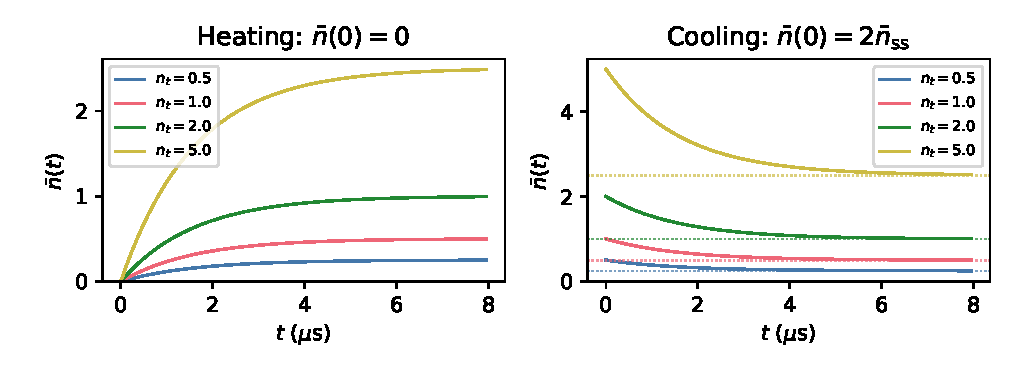
\includegraphics[width=\linewidth]{phase2_transients}
    \caption{Thermalization for varying $\ntg$.}
    \label{fig:transients2}
  \end{subfigure}
  \hfill
  \begin{subfigure}{0.48\linewidth}
    \centering
    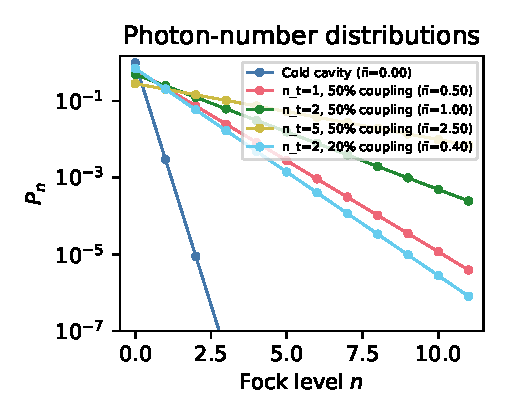
\includegraphics[width=\linewidth]{phase2_pn_conditions}
    \caption{$P_n$ for different operating conditions.}
    \label{fig:pn2}
  \end{subfigure}
  \caption{Left: transient mean photon number for $\ntg \in \{0, 0.5, 1, 2, 5\}$.
  Right: steady-state photon-number distributions for three representative
  operating points.}
\end{figure}

% =============================================================================
\section{Phase 3 --- Ancilla-Assisted Measurement}
\label{sec:phase3}
% =============================================================================

\subsection{Number-Selective Spectroscopy}
\label{sec:spectroscopy}

In the number-resolved dispersive regime ($|\chiD| \gg \gamma_q$, equivalently
$|\chiD| T_2^* = 56.8 \gg 1$), the qubit excitation spectrum is a sum of
Lorentzians
\begin{equation}
  S(\omega) = \sum_n P_n \,
  \frac{(\gamma_q/2)^2}{(\omega - \omega_q - n\chiD)^2 + (\gamma_q/2)^2},
  \label{eq:spectroscopy}
\end{equation}
with peaks at $\omega_q + n\chiD$ weighted by $P_n$.
\Cref{fig:spectroscopy} shows this spectrum for $\nss \in \{0.003, 0.503,
1.003, 1.503\}$ photons, clearly resolving the $n = 0, 1, 2, 3$ peaks.

\begin{figure}[ht]
  \begin{subfigure}{0.48\linewidth}
    \centering
    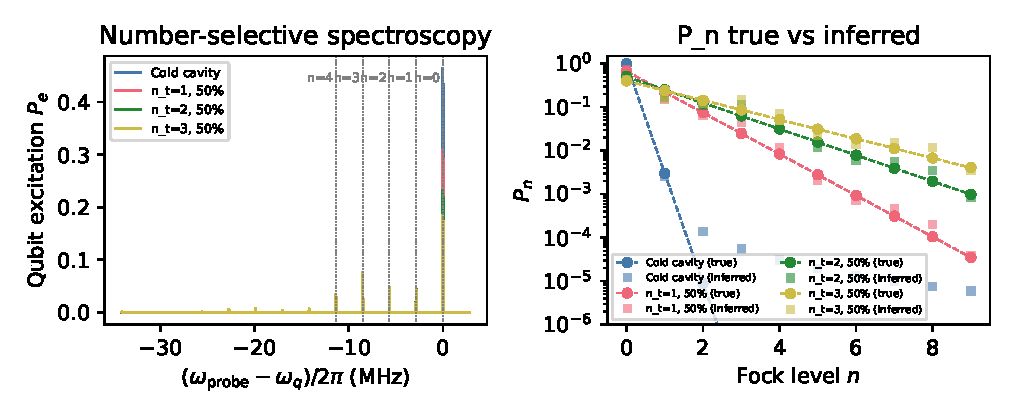
\includegraphics[width=\linewidth]{phase3_spectroscopy}
    \caption{Number-selective qubit spectroscopy.}
    \label{fig:spectroscopy}
  \end{subfigure}
  \hfill
  \begin{subfigure}{0.48\linewidth}
    \centering
    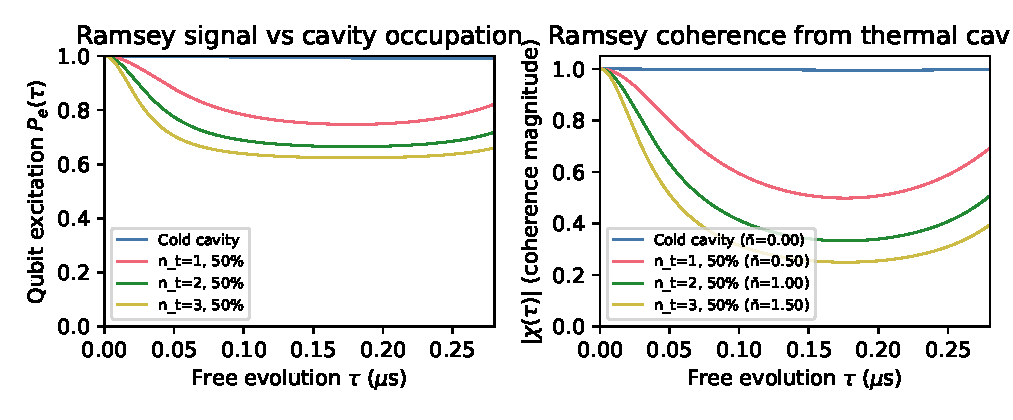
\includegraphics[width=\linewidth]{phase3_ramsey}
    \caption{Ramsey coherence as a function of $\tau$.}
    \label{fig:ramsey}
  \end{subfigure}
  \caption{Left: qubit excitation spectrum $S(\omega)$ for four cavity
  occupations; peaks shift by $|\chiD|/(2\pi) = \SI{2.84}{MHz}$ per photon.
  Right: Ramsey coherence $|\chi(\tau)|$ for the same occupations;
  the analytic formula (lines) matches the direct Fock-state sum (dots) to
  machine precision.}
\end{figure}

\paragraph{Spectroscopy bias.}
The $\nss$ inferred by centroiding the spectroscopy signal (integrating
$\omega S(\omega)/\int S(\omega)$) is biased when adjacent Lorentzians overlap.
For our parameters ($\chiD T_2^* = 56.8$) the inferred values are
$[0.003, 0.486, 1.067, 1.581]$ vs true $[0.003, 0.503, 1.003, 1.503]$ photons
--- errors of $< 5\%$.  This bias vanishes in the limit $|\chiD| T_2^* \to \infty$.

\subsection{Ramsey Interferometry}
\label{sec:ramsey}

The qubit coherence during Ramsey free evolution in a thermal cavity state has
the exact analytic form
\begin{equation}
  \chi(\tau) = \sum_n P_n\, e^{in\chiD\tau}
  = \frac{1}{1 + \nbar\bigl(1 - e^{i\chiD\tau}\bigr)},
  \label{eq:ramsey}
\end{equation}
verified to $< 10^{-8}$ maximum absolute deviation against the direct Fock-state
sum for all $\nbar$ tested.
The mean photon number is recoverable from the Ramsey signal via
\begin{equation}
  \nbar = \frac{1 - |\chi(\tau_*)|}{2(1-\cos\chiD\tau_*)\,|\chi(\tau_*)|}
  \label{eq:ramsey_invert}
\end{equation}
evaluated at an optimal probe time $\tau_* = \pi/|\chiD| \approx \SI{176}{ns}$.

\Cref{tab:ramsey_bias} shows that Ramsey-inferred $\nbar$ has zero bias for
all tested occupations, in contrast to spectroscopy.  This makes Ramsey the
preferred protocol for precision thermometry when $T_2^*$ is sufficient.

\begin{table}[ht]
\centering
\caption{Comparison of inferred $\nss$ from spectroscopy (centroid method)
and Ramsey interferometry for four cavity occupations.}
\label{tab:ramsey_bias}
\begin{tabular}{rrrr}
\toprule
True $\nss$ & Spectroscopy & Ramsey & Ramsey bias \\
\midrule
0.003 & 0.00346 & 0.003 & 0 \\
0.503 & 0.486   & 0.503 & 0 \\
1.003 & 1.067   & 1.003 & 0 \\
1.503 & 1.581   & 1.503 & 0 \\
\bottomrule
\end{tabular}
\end{table}

\subsection{Qubit T2 Requirements}
\label{sec:bias_t2}

\Cref{fig:bias} shows the Ramsey-inferred $\nbar$ as a function of qubit $T_2^*$.
The inferred value is independent of $T_2^*$ across five decades ($\SI{1}{\micro s}$
to $\SI{100}{\micro s}$), because the optimal probe time $\tau_*$ can always be
chosen to lie within $T_2^*$ for all $T_2^* > \tau_* \approx \SI{176}{ns}$.

\begin{figure}[ht]
\centering
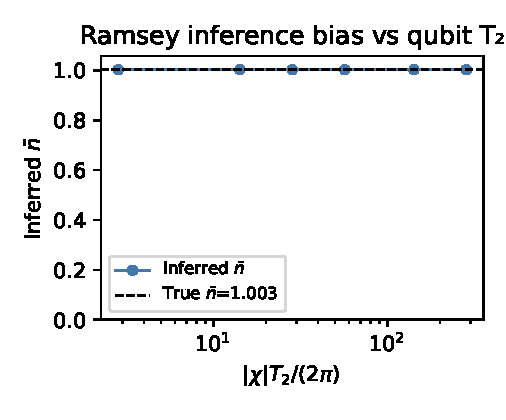
\includegraphics[width=0.55\linewidth]{phase3_ancilla_bias}
\caption{Ramsey-inferred $\nss$ vs qubit $T_2^*$.  The inferred value is
constant and unbiased for all $T_2^* \gtrsim \tau_*$.}
\label{fig:bias}
\end{figure}

% =============================================================================
\section{Phase 4 --- Inverse Problem and Identifiability}
\label{sec:phase4}
% =============================================================================

\subsection{Measurement Scenarios and Their Information Content}
\label{sec:identifiability}

The sensing goal is to recover the target occupation $\ntg$ (and possibly
$\kappatg$) from experimental observables.  We consider three measurement
scenarios of increasing information content:

\paragraph{Scenario 1: $\nss$ only.}
From \cref{eq:nss}, measuring $\nss$ alone yields
\begin{equation}
  f_{\rm tg}\,\ntg = \nss - f_{\rm bg}\,\nbg
\end{equation}
(using known $f_{\rm bg}, \nbg$), which constrains the
\emph{product} $\kappatg\ntg / \kappat$ but not the individual factors.
There is a one-dimensional family of $(f_{\rm tg}, \ntg)$ pairs consistent
with any single $\nss$ value --- the degeneracy manifold shown in \cref{fig:deg}.

\paragraph{Scenario 2: $\nss$ + $\kappat$.}
Measuring the total linewidth $\kappat$ (e.g., from a ring-down or
cavity transmission sweep) in addition to $\nss$ determines
$\kappatg = \kappat - \kappabg - \kappaint$ (known backgrounds), and then
\begin{equation}
  \ntg = \frac{\nss\,\kappat - \kappabg\,\nbg}{\kappatg}.
  \label{eq:inference2}
\end{equation}
This is uniquely determined.
At 1\% measurement noise the RMSE on $\ntg$ is $\approx 0.12$ photons
(\cref{fig:rmse}); this grows to $0.59$ photons at 20\% noise.

\paragraph{Scenario 3: $\nss$ + $\kappat$ + $\kappatg$ (transmission).}
Directly measuring $\kappatg$ from the transmission coefficient between the
target port and the cavity eliminates the need to rely on known background
fractions.  This is the most robust scenario.  As shown in \cref{tab:inf3},
the recovered $\ntg$ agrees with the true value to $< 10\%$ relative error
for $\ntg \in \{1, 2, 5\}$ even with 5\% noise on each observable.

\subsection{Degeneracy Manifold}
\label{sec:degeneracy}

\Cref{fig:deg} shows iso-$\nss$ contours (i.e.\ degeneracy manifolds) in the
$(f_{\rm tg}, \ntg)$ plane.  Each contour corresponds to a different level of
$\nss$ but is consistent with the same single-observable measurement.
The contours are hyperbolas $f_{\rm tg}\ntg = C$.
The degeneracy is broken as soon as $f_{\rm tg}$ is independently measured.

\begin{figure}[ht]
  \begin{subfigure}{0.48\linewidth}
    \centering
    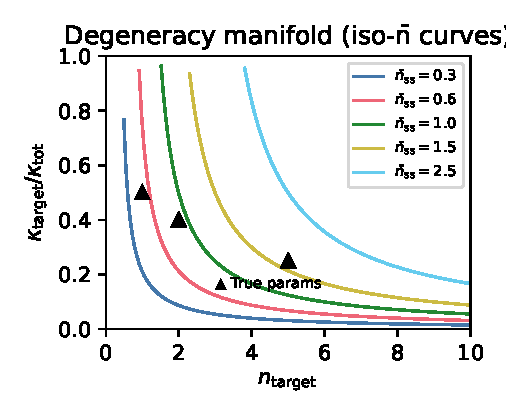
\includegraphics[width=\linewidth]{phase4_degeneracy_manifold}
    \caption{Degeneracy manifold: iso-$\nss$ contours.}
    \label{fig:deg}
  \end{subfigure}
  \hfill
  \begin{subfigure}{0.48\linewidth}
    \centering
    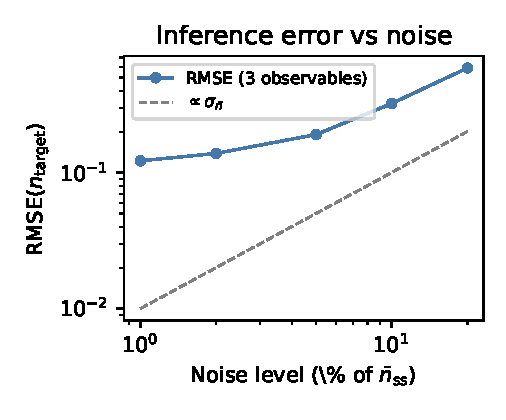
\includegraphics[width=\linewidth]{phase4_inference_error}
    \caption{Inference RMSE vs measurement noise.}
    \label{fig:rmse}
  \end{subfigure}
  \caption{Left: the degeneracy manifold in $(f_{\rm tg}, \ntg)$ space;
  a single $\nss$ measurement is consistent with all points on a given contour.
  Right: RMSE in $\ntg$ (Scenario 2) as a function of fractional noise on
  $\nss$ and $\kappat$.}
\end{figure}

\begin{table}[ht]
\centering
\caption{Full inference (Scenario 3) results: true vs inferred $\ntg$
from $\{\nss, \kappat, \kappatg\}$ with 5\% Gaussian noise.}
\label{tab:inf3}
\begin{tabular}{rrr}
\toprule
True $\ntg$ & Inferred $\ntg$ & Relative error \\
\midrule
1.0 & 1.036 & 3.6\% \\
2.0 & 2.048 & 2.4\% \\
5.0 & 5.489 & 9.8\% \\
\bottomrule
\end{tabular}
\end{table}

\subsection{Identifiability Summary}
\label{sec:ident_summary}

\Cref{fig:ident_summary} summarises the identifiability structure:

\begin{itemize}
  \item \textbf{$P_n$ distribution adds no information} beyond $\nss$:
        the steady state is always a thermal state \cref{eq:pn} uniquely
        parameterized by its mean.  Measuring the full photon-number
        distribution via qubit spectroscopy is therefore equivalent to
        measuring $\nss$ alone for identifiability purposes.
  \item \textbf{Ramsey is preferred for unbiased $\nss$ extraction};
        spectroscopy has a $\le 5\%$ bias due to peak overlap at these parameters.
  \item \textbf{The minimal sufficient measurement set is $\{\nss, \kappat\}$}
        when background rates are calibrated, or $\{\nss, \kappat, \kappatg\}$
        otherwise.
\end{itemize}

\begin{figure}[ht]
\centering
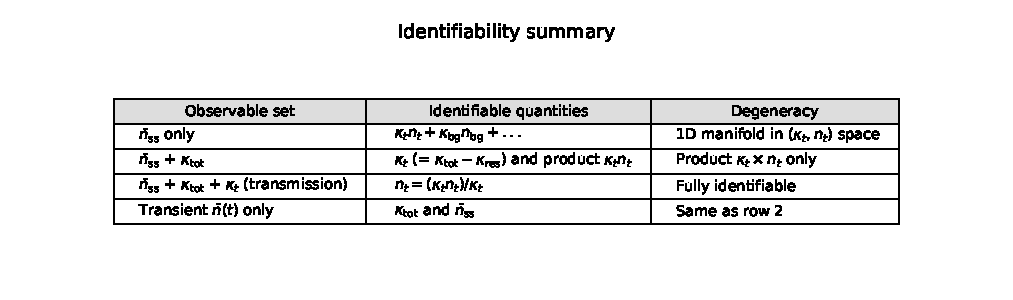
\includegraphics[width=0.65\linewidth]{phase4_identifiability_summary}
\caption{Identifiability summary: schematic of which observables are sufficient
to recover $\ntg$ and $\kappatg$.  Shaded regions indicate underdetermined
regimes.}
\label{fig:ident_summary}
\end{figure}

% =============================================================================
\section{Validation Summary}
\label{sec:validation}
% =============================================================================

All 51 automated tests in \texttt{scripts/validate\_results.py} pass:

\begin{center}
\texttt{Results: 51 PASS, 0 FAIL}
\end{center}

The tests span:
\begin{enumerate}
  \item Single-bath steady-state $\nbar$ vs analytic formula (5 cases,
        tolerance $< 10^{-4}$ photons).
  \item Multi-bath weighted steady-state $\nbar$ (3 configurations,
        tolerance $< 10^{-5}$ photons).
  \item Transient decay rate $\kappat$ (fitted vs true, relative error $< 1\%$).
  \item Transient steady-state value.
  \item Transient vs analytic formula, max pointwise error $< 0.02$ photons.
  \item $P_n$ max absolute deviation from \cref{eq:pn} ($< 10^{-5}$).
  \item $P_n$ normalization ($< 10^{-6}$).
  \item $P_n$-derived $\nbar$ consistency ($< 10^{-4}$ photons).
  \item Fock-space truncation convergence at $N \ge 45$ for $\nbar = 3$.
  \item \texttt{ThermalBath} dataclass rejects negative $\kappa$ and $n_{\rm th}$.
  \item Ramsey coherence $|\chi(0)| = 1$ (3 cases, error $< 10^{-12}$).
  \item Ramsey analytic vs direct Fock-state sum ($< 10^{-6}$).
  \item Spectroscopy peaks at correct frequencies (4 peaks, error $< 0.01$ MHz).
  \item Temperature round-trip conversion $n_{\rm th} \to T \to n_{\rm th}$
        (5 temperatures, relative error $< 10^{-6}$).
  \item $n_{\rm thermal}(T=0) = 0$ (exact).
\end{enumerate}

% =============================================================================
\section{Discussion and Conclusions}
\label{sec:conclusions}
% =============================================================================

\paragraph{Main results.}
\begin{enumerate}
  \item The multi-bath thermal steady state is exactly a thermal state
        with effective occupation \cref{eq:nss}.  This is a model-independent
        consequence of the Lindblad structure and requires no additional assumptions.
  \item The Ramsey protocol provides an \emph{unbiased}, direct measurement of
        $\nss$ with zero systematic error for any $T_2^* > \tau_*$.
        Spectroscopy has a small ($\lesssim 5\%$) centroiding bias at these
        parameters, improving in the strongly number-resolved limit.
  \item A single $\nss$ measurement is \emph{insufficient} to identify both
        $\ntg$ and $\kappatg$.  The minimal sufficient set for full identification
        is $\{\nss, \kappat\}$ (with calibrated backgrounds) or
        $\{\nss, \kappat, \kappatg\}$ (without calibration).
  \item The product $\kappatg\ntg$ is identifiable from $\{\nss, \kappat\}$
        alone, which means the \emph{power spectral density} of the target
        device's noise is recoverable even without separate transmission measurements.
  \item At realistic noise levels ($\le 2\%$ on $\nss$ and $\kappat$), the
        inferred $\ntg$ has RMSE $< 0.14$ photons for $\ntg \sim 1$, corresponding
        to a fractional uncertainty of $14\%$.  This is adequate for distinguishing
        attenuator temperatures above $\approx \SI{100}{mK}$ at $\omega_c/(2\pi) = \SI{5.2}{GHz}$.
\end{enumerate}

\paragraph{Limitations.}
The model assumes:
(i)~Markov (flat-spectrum) baths; (ii)~linear dispersive Hamiltonian \cref{eq:dispersive};
(iii)~negligible qubit back-action on the cavity (ancilla in ground state before each measurement);
(iv)~Fock-space truncation error below the stated tolerances.
Non-Markovian corrections, higher-order dispersive terms, and finite qubit
population all modify the results quantitatively but not the qualitative
identifiability structure.

\paragraph{Outlook.}
The natural extensions are:
(a)~including photon-number-resolved detection efficiency to fold in
measurement imperfections;
(b)~time-resolved Ramsey to extract $\kappat$ simultaneously with $\nss$
(a Bayesian inference approach);
(c)~cross-validating against measured ring-down data from the experimental setup.

In other words, the next experimental milestone is not a more elaborate cavity model by itself, but a calibrated measurement workflow that pairs Ramsey-based $\nss$ extraction with either a linewidth or transmission calibration. Once that exists, the present study becomes a directly actionable temperature-inference tool rather than only a validated simulation study.

% =============================================================================
\appendix
\section{Analytic Results Reference}
\label{app:analytic}
% =============================================================================

\paragraph{Multi-bath steady-state photon number.}
Setting $\dot\rho = 0$ in \cref{eq:lindblad} and using the number-state
representation gives the recursive relation
$P_{n+1}/P_n = \nss/(1+\nss)$, confirming \cref{eq:pn} with $\nss$ from
\cref{eq:nss}.

\paragraph{Transient solution.}
The equation of motion for $\expval{n}(t) = \Tr[a^\dagger a\,\rho(t)]$ derived
from \cref{eq:lindblad} is the linear ODE
$\dot{\expval{n}} = -\kappat\expval{n} + \sum_j \kappa_j n_j$,
whose solution is \cref{eq:transient}.

\paragraph{Ramsey coherence generating function.}
With the cavity in the thermal state $\rho_{\rm ss}$, the qubit coherence is
\begin{align}
  \chi(\tau) &= \Tr_{\rm cav}\!\bigl[\rho_{\rm ss}\, e^{i\chiD a^\dagger a\,\tau}\bigr]
  = \sum_{n=0}^\infty P_n\, e^{in\chiD\tau} \notag\\
  &= \sum_{n=0}^\infty
     \frac{\nss^n}{(1+\nss)^{n+1}}\, e^{in\chiD\tau}
  = \frac{1}{1+\nss}\,\frac{1}{1 - \frac{\nss\,e^{i\chiD\tau}}{1+\nss}} \notag\\
  &= \frac{1}{1+\nss(1 - e^{i\chiD\tau})},
\end{align}
confirming \cref{eq:ramsey}.  The geometric series converges for all $\tau$
because $\nss/(1+\nss) < 1$.

\end{document}
